\documentclass{ximera}
\input{../preamble.tex}

\title{Challenge Problems for Ch 5} \license{CC BY-NC-SA 4.0}

\begin{document}

\begin{abstract}
\end{abstract}
\maketitle

\section*{Challenge Problems for Chapter 5}

\begin{problem}\label{prob:rotLinTransGeom}
    Argue geometrically to prove that the following transformations are linear:
\begin{enumerate}
\item Rotation of the plane about the origin through angle $\theta$.
\item Reflection of the plane about the line $y=mx$.
\end{enumerate}
\begin{hint}
Think in terms of linearity diagrams.
\begin{center}
 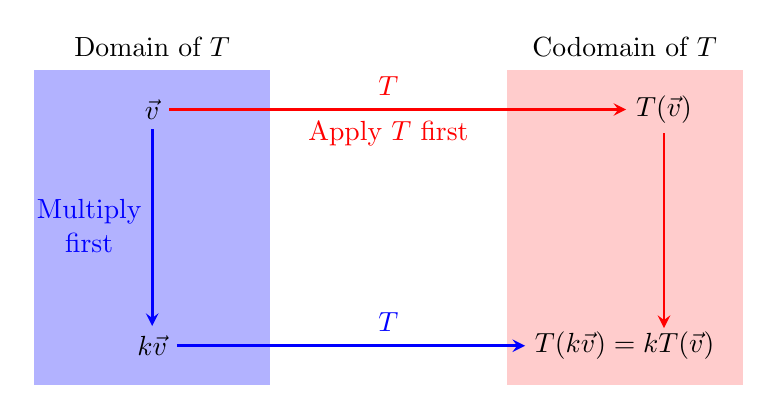
\begin{tikzpicture} 
      
    \fill[blue, opacity=0.3] (1,1) rectangle (4,5);
   \fill[red, opacity=0.2] (7,1) rectangle (10,5);
   
   \node[] at (2.5, 5.3)  (p2)    {Domain of $T$};
   \node[] at (8.5, 5.3)  (r3)    {Codomain of $T$};
   
      \node[] at (2.5, 4.5)  (a)    {$\vec{v}$};
     \node[] at (2.5, 1.5)  (b)    {$k\vec{v}$};
     
    
    \node[] at (9, 4.5)  (c)    {$T(\vec{v})$};
     \node[] at (8.5, 1.5)  (d)    {$T(k\vec{v})=kT(\vec{v})$};
     \node[] at (9, 1.6)  (e) {};
     
    
     \draw [->,line width=1pt,-stealth, red]  (a.east)to(c.west);
     \draw [->,line width=1pt,-stealth, blue]  (b.east)to(d.west);
     
     \draw [->,line width=1pt,-stealth, blue]  (a.south)to(b.north);
     \draw [->,line width=1pt,-stealth,red]  (c.south)to(e.north);
     
%Function labels
      \node[red] at (5.5, 4.8)    {$T$};
      \node[blue] at (5.5, 1.8)    {$T$};
      
      \node[blue] at (1.7, 3.2)    {Multiply};
      \node[blue] at (1.7, 2.8)    {first};
      \node[red] at (5.5, 4.2)    {Apply $T$ first};   
      
  \end{tikzpicture}
\end{center}

\begin{center}
 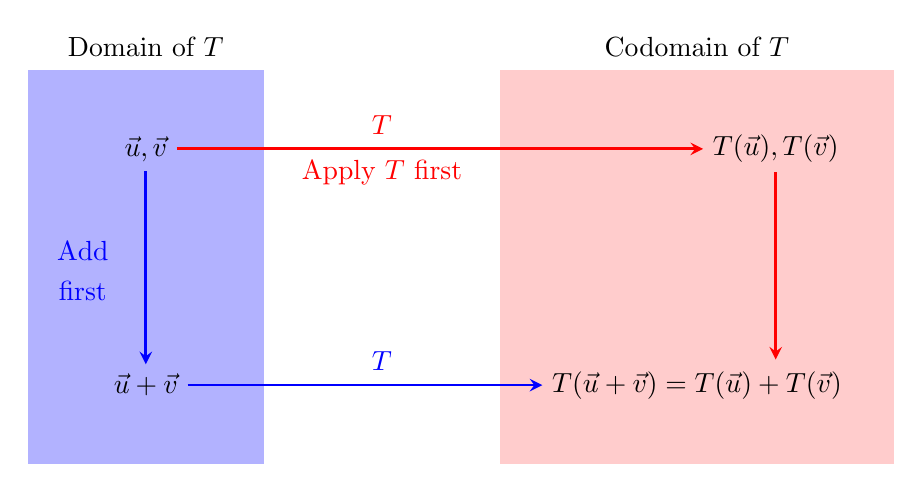
\begin{tikzpicture} 
      
    \fill[blue, opacity=0.3] (1,1) rectangle (4,6);
   \fill[red, opacity=0.2] (7,1) rectangle (12,6);
   
   \node[] at (2.5, 6.3)  (p2)    {Domain of $T$};
   \node[] at (9.5, 6.3)  (r3)    {Codomain of $T$};
   
      \node[] at (2.5, 5)  (a)    {$\vec{u}, \vec{v}$};
     \node[] at (2.5, 2)  (b)    {$\vec{u}+\vec{v}$};
     
    
    \node[] at (10.5, 5)  (c)    {$T(\vec{u}),T(\vec{v})$};
     \node[] at (9.5, 2)  (d)    {$T(\vec{u}+\vec{v})=T(\vec{u})+T(\vec{v})$};
     \node[] at (10.5, 2.2)  (e) {};
     
    
     \draw [->,line width=1pt,-stealth, red]  (a.east)to(c.west);
     \draw [->,line width=1pt,-stealth, blue]  (b.east)to(d.west);
     
     \draw [->,line width=1pt,-stealth, blue]  (a.south)to(b.north);
     \draw [->,line width=1pt,-stealth,red]  (c.south)to(e.north);
     
%Function labels
      \node[red] at (5.5, 5.3)    {$T$};
      \node[blue] at (5.5, 2.3)    {$T$};
      
      \node[blue] at (1.7, 3.7)    {Add};
      \node[blue] at (1.7, 3.2)    {first};
      \node[red] at (5.5, 4.7)    {Apply $T$ first};   
      
  \end{tikzpicture}
\end{center}
What happens when you rotate two vectors first, then add them, versus adding the two vectors first, then rotating the sum?  

The figure below illustrates the left side of the diagram.  Vectors $\vec{u}$ and $\vec{v}$ are added in the domain, then the sum is rotated through angle $\theta$.


\begin{center}

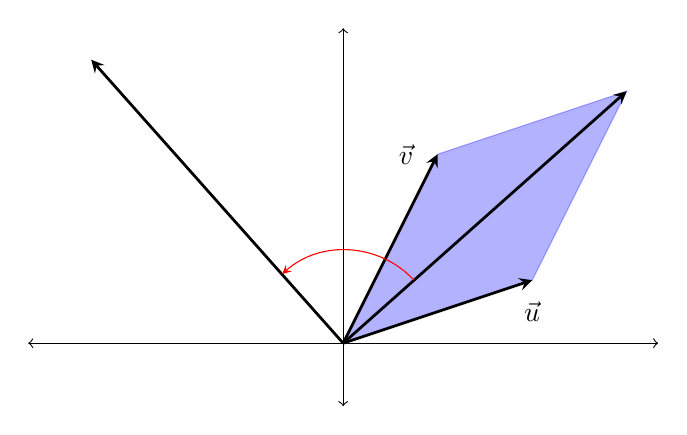
\begin{tikzpicture}[scale=0.8]

  \draw[<->] (-5,0)--(5,0);
  \draw[<->] (0,-1)--(0,5);
  \filldraw[blue, opacity=0.3](0,0)--(3,1)--(4.5,4)--(1.5,3)--cycle;
  \draw[->,line width=1pt,-stealth](0,0)--(3,1);
   \draw[->,line width=1pt,-stealth](0,0)--(1.5,3);
    \draw[->,line width=1pt,-stealth](0,0)--(4.5,4);
    \node[] at (3, 0.5)   (k1u) {$\vec{u}$};
    \node[] at (1, 3)   (k2v) {$\vec{v}$};
    \draw[->,line width=1pt,-stealth](0,0)--(-4,4.5);
    \draw[->,red,-stealth] (4.5/4,1) arc (43:131.6:1.5) ;
    \end{tikzpicture}
\end{center} 

The next figure  illustrates what happens when vectors $\vec{u}$ and $\vec{v}$ are rotated through angle $\theta$, then their images are added together.  

\begin{center}
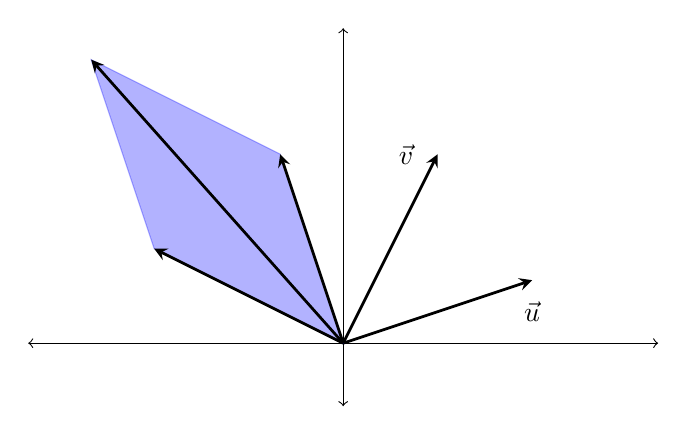
\begin{tikzpicture}[scale=0.8]

  \draw[<->] (-5,0)--(5,0);
  \draw[<->] (0,-1)--(0,5);
  \draw[->,line width=1pt,-stealth](0,0)--(3,1);
  \draw[->,line width=1pt,-stealth](0,0)--(1.5,3);
    \node[] at (3, 0.5)   (k1u) {$\vec{u}$};
    \node[] at (1, 3)   (k2v) {$\vec{v}$};
  % \draw[->,red,-stealth] (4.5/4,1) arc (70:148.6:1.5) ;
  \filldraw[blue, opacity=0.3](0,0)--(-1,3)--(-4,4.5)--(-3,1.5)--cycle;
  \draw[->,line width=1pt,-stealth](0,0)--(-1,3);
   \draw[->,line width=1pt,-stealth](0,0)--(-3,1.5);
   \draw[->,line width=1pt,-stealth](0,0)--(-4,4.5);
    \end{tikzpicture}
  \end{center}
  
  
  Because the diagonal of a parallelogram rotates with the parallelogram, it is clear that 
$$R_{\theta}(\vec{u}+\vec{v})=R_{\theta}(\vec{u})+R_{\theta}(\vec{v})$$
\end{hint}
\end{problem}

\begin{problem}\label{prb:6.25} Find the matrix of the linear transformation which rotates every
vector in $\mathbb{R}^{3}$ counter clockwise about the $z$ axis when viewed
from the positive $z$ axis through an angle of 30$^{\circ }$ and then
reflects through the $xy$ plane.

Click on the arrow to see answer.
\begin{expandable}
\[
\left[
\begin{array}{rrr}
1 & 0 & 0 \\
0 & 1 & 0 \\
0 & 0 & -1
\end{array}
\right] \left[
\begin{array}{ccc}
\cos \left( \frac{\pi }{6}\right)  & -\sin \left( \frac{\pi }{6}\right)  & 0
\\
\sin \left( \frac{\pi }{6}\right)  & \cos \left( \frac{\pi }{6}\right)  & 0
\\
0 & 0 & 1
\end{array}
\right] = \left[
\begin{array}{ccc}
\frac{1}{2}\sqrt{3} & -\frac{1}{2} & 0 \\
\frac{1}{2} & \frac{1}{2}\sqrt{3} & 0 \\
0 & 0 & -1
\end{array}
\right]
\]
\end{expandable}
\end{problem}

\begin{problem}\label{prob:imAndKer0}
    Let $T:\RR^n\rightarrow \RR^m$ be a linear transformation such that $\text{ker}(T)=\RR^n$.  Find $\text{im}(T)$.
\end{problem}

\begin{problem}\label{prob:nich7.1.13}
    Let $\vec{v}$ be a non-zero vector in $\RR^n$.  Given any vector $\vec{w}$ in $\RR^m$, show there exists a linear transformation $T:\RR^n\rightarrow\RR^m$ with $T(\vec{v})=\vec{w}$.
\end{problem}

\begin{problem}\label{prob:nich7.1.14}
    Given $\vec{y}$ in $\RR^n$, define $S_{\vec{y}}:\RR^n\rightarrow\RR$ by $S_{\vec{y}}(\vec{x})=\vec{x}\dotp\vec{y}$ for all $\vec{x}$ in $\RR^n$.  
    \begin{enumerate}
        \item Show that $S_{\vec{y}}$ is a linear transformation.
        \item Show that every linear transformation $T:\RR^n\rightarrow\RR$  arises in this way (i.e. $T=S_{\vec{y}}$ for some $\vec{y}$ in $\RR^n$.)
    \end{enumerate}
    \begin{hint}
        Write $S_{\vec{y}}(\vec{e}_i)=y_i$ for $i=1,\dots , n$.
    \end{hint}
    
\end{problem}




\section*{Bibliography}
Some of these problems come from Chapter 5 of Ken Kuttler's \href{https://open.umn.edu/opentextbooks/textbooks/a-first-course-in-linear-algebra-2017}{\it A First Course in Linear Algebra}. (CC-BY)

Ken Kuttler, {\it  A First Course in Linear Algebra}, Lyryx 2017, Open Edition, pp. 272--315.   

Some of these problems come from the end of Chapter 7 of Keith Nicholson's \href{https://open.umn.edu/opentextbooks/textbooks/linear-algebra-with-applications}{\it Linear Algebra with Applications}. (CC-BY-NC-SA)

W. Keith Nicholson, {\it Linear Algebra with Applications}, Lyryx 2018, Open Edition, pp. 376--386. 



\end{document}